%=========================================================

% Here you can choose to compile with or without solutions.
% However, this definition is ignored if you use any
% command from the `Makefile`.
\providecommand{\withSol}{\iftrue}

%=========================================================

\documentclass
[twoside,english,colorbacktitle,accentcolor=tud9c]
{tudexercise}

\usepackage[T1]{fontenc}
\usepackage[latin9]{inputenc}
\usepackage{amstext}
\usepackage{amsmath}
\usepackage{graphicx}
\usepackage{setspace}
\usepackage{multicol}
\usepackage{mathtools}
\usepackage{dsfont}
\usepackage{units}
\usepackage{subfigure}
\usepackage{color}
\usepackage{booktabs}
\usepackage{fancyref}
\usepackage[ngerman,english]{babel}

%=========================================================

\def\homework{2}
\def\homeworkVer{1}
\def\homeworkSolVer{1}
\def\lecture{Machine Learning}
\def\semester{Summer Semester 2019}
\def\prof{Prof. Dr. J. Peters, H. Abdulsamad, S. Stark, D. Koert}
\def\deadline{Due date: Friday, 14 June 2019 17:00 \\
Hand in a PDF over Moodle \textbf{and} a printed version to the postbox at (S2/02 | E315)}

%=========================================================

\ifcsname withSol\endcsname\else
  \expandafter\let\csname withSol\expandafter\endcsname
                  \csname iffalse\endcsname
\fi

\withSol
	\usepackage[solutions]{iasHomework}
\else
	\usepackage{iasHomework}
\fi

%=========================================================

% USE YOUR NAMES!
\newcommand{\studentdata}{}
%\newcommand{\studentdata}{John Doe, 1234567 \qquad Jane Doe, 7654321}

\begin{document}
	
	\hwtitle{}
	\maketitle
	
	\begin{examheader}
		\normalsize
		\vspace{-1em}
		Name, Surname, ID Number \hfill \studentdata{}
		\vspace{-1em}
	\end{examheader} 
	
	\textbf{Name, Surname, ID Number \hfill \studentdata{}}

	\newif\ifvimbug
\vimbugfalse

\ifvimbug
\begin{document}
\fi

\exercise{Bayesian Decision Theory}
In this exercise, we consider data generated by a mixture of two Gaussian distributions with parameters $\{\mu_1$, $\sigma_1\}$ and $\{\mu_2$, $\sigma_2\}$. Each Gaussian represents a class labeled $C_1$ and $C_2$, respectively. 

\begin{questions}

%----------------------------------------------

\begin{question}{Optimal Boundary}{4}
Explain in one short sentence what Bayesian Decision Theory is. What is its goal? 
What condition does hold at the optimal decision boundary? When do we decide for class $C_1$ over $C_2$?

\begin{answer}\end{answer}

\end{question}


%----------------------------------------------

\begin{question}{Decision Boundaries}{8}
If both classes have equal prior probabilities $p(C_1) = p(C_2)$ and the same variance $\sigma_1 = \sigma_2$, derive the decision boundary $x^*$ analytically as a function of the two means $\mu_1$ and $\mu_2$.

\begin{answer}\end{answer}

\end{question}

%----------------------------------------------

\begin{question}{Different Misclassification Costs}{8}
Assume $\mu_1 > 0$, $\mu_1 = 2\mu_2$, $\sigma_1=\sigma_2$ and $p(C_1) = p(C_2)$. If misclassifying sample $x \in C_2$ as class $C_1$ is three times more expensive than the opposite, how does the decision boundary change? Derive the boundary analytically.
(There is no cost for correctly classifying samples.)

\begin{answer}\end{answer}

\end{question}

%----------------------------------------------

\end{questions}

	
	\newif\ifvimbug
\vimbugfalse

\ifvimbug
\begin{document}
\fi

\exercise{Density Estimation}
In this exercise, you will use the datasets \texttt{densEst1.txt} 
and \texttt{densEst2.txt}. The datasets contain 2D data belonging
to two classes, $C_1$ and $C_2$.

\begin{questions}

%----------------------------------------------

\begin{question}{Gaussian Maximum Likelihood Estimation}{10}
Derive the ML estimate for the mean and covariance of the \textbf{multivariate} Gaussian distribution. Start your derivations with the function you optimize. Assume that you can collect i.i.d data. (Hint: you can find many matrix identities on the Matrix Cookbook (\url{https://www.math.uwaterloo.ca/~hwolkowi/matrixcookbook.pdf}) and at \url{http://en.wikipedia.org/wiki/Matrix_calculus}.)

\begin{answer}
The Multivariate Gaussian Distribution is defined as

\begin{equation}
	f_x(\mu|\Sigma) = \frac{1}{\sqrt{(2\pi)^p \text{det}(\Sigma)}} \text{exp} (-\frac{1}{2}(x-\mu)^T \Sigma^{-1} (x-\mu))
\end{equation}

$\Sigma$ is the Covariance Matrix defined as:
\begin{equation}
\begin{pmatrix}
	\sigma_{xx}^2 & \sigma_{xy}^2 \\
	\sigma_{xy}^2 & \sigma_{yy}^2 \\
\end{pmatrix}
\end{equation}

The resulting likelihood function of $f_x(x)$ is:

\begin{equation}
L(\mu, \Sigma) = \prod\limits_{n=1}^{N} f_x(\mu|\Sigma)
\end{equation}

We now take the log of the likelihood function.

\begin{equation}
	\log L(\mu, \Sigma) = \sum_{n=1}^{N} \log f_x(\mu|\Sigma)
\end{equation}

Resulting in the log likelihood function for a multivariate gausian distribution.

\begin{equation} \label{L}
	\log L(\mu, \Sigma) = \sum_{n=1}^{N} \log (\frac{1}{\sqrt{(2\pi)^p \text{det}(\Sigma)}} \text{exp} (-\frac{1}{2}(x-\mu)^T \Sigma^{-1} (x-\mu)))
\end{equation}

Now we want to derive the mean and covariance for this distribution. Starting with the mean, we need to maximize the partial equation.

\begin{equation}
\frac{\partial L }{\partial \mu} = \sum_{n=1}^{N} \underbrace{\log (\frac{1}{\sqrt{(2\pi)^p \text{det}(\Sigma)}})'}_{0} +
\sum_{n=1}^{N} (-\frac{1}{2}(x-\mu)^T \Sigma^{-1} (x-\mu))'
\end{equation}

For matrix Calculus we use following rules:
\begin{equation}
\frac{\partial(Xa+b)^T C(Xa+b)}{\partial x} = (C+C^T) (Xa +b)a^T
\end{equation}

With $X = x$, $a = 1$, thus $a^T = 1$ and $b = -\mu$. We get

\begin{equation}
\sum_{n=1}^{N} (\Sigma + (\Sigma^{-1})^T (x - \mu)) = 0
\end{equation}

Since $\Sigma$ is a symmetrical Matrix $\Sigma + \Sigma^T = 2\cdot\Sigma$ holds true. This matrix is also constant, meaning its independend on the sum and can be written before it.

\begin{equation}
2\Sigma^{-1} \cdot \sum_{n=1}^{N} (x-\mu) = 0
\end{equation}
\begin{equation}
\sum_{n=1}^{N}x_i = \sum_{n=1}^{N}\mu
\end{equation}

Since $\mu$ is a constant we can write the sum over a constant as $N\cdot\mu$
\begin{equation}
\sum_{n=1}^{N}x_i = N\cdot\mu
\end{equation}

Resulting in the following equation for the mean:
\begin{equation}
\mu = \frac{1}{N} \sum_{n=1}^{N}x_i
\end{equation}

Now we want to derive the maximum Likelihood estimate for the covariance of the multivariate Gaussian distribution. Again we Start with Equation \eqref{L}.
For this derivation the will the following rules for matrix calculus.
\begin{equation}
	\frac{\partial}{\partial A} \log(\det(A)) = (A^{-1})^T
\end{equation}
\begin{equation}
	\frac{\partial}{\partial A}x^T A x = xx^T
\end{equation}
With $A = \Sigma$ and $x = (x-\mu)$.
First we split the log of gaussian equation up into three part for easier derivation.

\begin{equation}
\frac{\partial L}{\partial \Sigma} = \underbrace{\log(\frac{1}{\sqrt{2\pi}^P})'}_{\text{a}} + \sum_{n=1}^{N}(\underbrace{\log(\frac{1}{\sqrt{\det(\Sigma)}})'}_{b} + \underbrace{\log \exp (-\frac{1}{2} (x-\mu)^T \Sigma^{-1}(x-\mu))'}_{c})
\end{equation}

For $a$:
\begin{equation}
	\frac{\partial L_a}{\partial \Sigma} = 0
\end{equation}

For $b$:
\begin{equation}
	\log(\frac{1}{\sqrt{\det(\Sigma)}}) = \log(\frac{1}{\det(\Sigma)^{\frac{1}{2}}}) = \frac{1}{2}\cdot\log(\frac{1}{\det(\Sigma)})
\end{equation}

\begin{equation}
\frac{\partial L_b}{\partial \Sigma} = \frac{1}{2}\cdot\frac{1}{(\Sigma^{-1})^T} = \frac{1}{2} \cdot \Sigma
\end{equation}

For $c$:
\begin{equation}
	\frac{\partial L_c}{\partial \Sigma} = -\frac{1}{2}(x - \mu)\cdot(x - \mu)^T
\end{equation}

In total we get the following derivative:
\begin{equation}
	\frac{\partial L}{\partial \Sigma} = \sum_{n=1}^{N}\frac{1}{2}\Sigma - \sum_{n=1}^{N}(\frac{1}{2}(x - \mu)\cdot(x - \mu)^T) = 0
\end{equation}

Multiplied by $\frac{1}{2}$:
\begin{equation}
	\sum_{n=1}^{N} \Sigma = \sum_{n=1}^{N}((x - \mu)\cdot(x - \mu)^T)
\end{equation}

Since $\Sigma$ is constant we can write $\sum_{n=1}^{N}\Sigma = N\cdot\Sigma$.
Resulting in the final equation for the covariance
\begin{equation}
	\Sigma = \frac{1}{N} \sum_{n=1}^{N}(x_i -\mu)\cdot(x_i - \mu)^T
\end{equation}

\end{answer}

\end{question}

%----------------------------------------------

\begin{question}{Prior Probabilities}{2}
Compute the prior probability of each class from the dataset. 

\begin{answer}
We count for class 1: $n_1 = 239$ and for class 2: $n_2 = 761$. Resulting in following priors
\begin{equation}
	p(C_1) = \frac{239}{239+761} = 0.239
\end{equation}
\begin{equation}
    p(C_2) = \frac{761}{239+761} = 0.761
\end{equation}

\end{answer}

\end{question}


%----------------------------------------------

\begin{question}{Biased ML Estimate}{5}
Define the bias of an estimator and write how we can compute it.
Then calculate the biased and unbiased estimates of the conditional distribution $p(x|C_i)$, assuming that each class can be modeled with a Gaussian distribution. Which parameters have to be calculated?
Show the final result and attach a snippet of your code.
Do not use existing functions, but rather implement the computations by yourself!

\begin{answer}
The bias of an estimator $\Theta$ measures the difference between the expected value of an estimator and its' true value. It is is defined as:
\begin{equation*}
Bias(\widehat{\theta})= E(\widehat{\theta}) - \theta
\end{equation*}
Assuming a Gaussian distribution, the biased and unbiased estimates of the conditional distributions can be calculated using the following formula:
\begin{align*}
&\overline{\mathbf{x}}_{unbiased}= \frac{1}{N} \sum_{i=1}^{n} \mathbf{x}_{i} \\
&\widehat{\boldsymbol{\Sigma}}_{unbiased}=\frac{1}{N-1} \sum_{i=1}^{N}(\mathbf{x}_{i}-\overline{\mathbf{x}})(\mathbf{x}_{i}-\overline{\mathbf{x}})^{\mathrm{T}} \\
&\widehat{\boldsymbol{\Sigma}}_{biased}=\frac{1}{N} \sum_{i=1}^{N}(\mathbf{x}_{i}-\overline{\mathbf{x}})(\mathbf{x}_{i}-\overline{\mathbf{x}})^{\mathrm{T}}
\end{align*}
We thus obtain the following values for the given dataset.
\begin{align*}
&\overline{\mathbf{x}}_{1, unbiased} =  
\begin{bmatrix} 
-0.70681374 \\
 -0.81343083
\end{bmatrix}\\
&\widehat{\boldsymbol{\Sigma}}_{1, unbiased} =
\begin{bmatrix} 
9.05742302 & 2.6841014 \\
2.6841014 & 3.61145033 
\end{bmatrix}
\\
&\widehat{\boldsymbol{\Sigma}}_{1, biased} =
\begin{bmatrix} 
9.01952586 & 2.67287085 \\
2.67287085 & 3.59633965 
\end{bmatrix}
\\
&\overline{\mathbf{x}}_{2, unbiased} =
\begin{bmatrix} 
3.98534252 \\
3.98438364
\end{bmatrix}\\
&\widehat{\boldsymbol{\Sigma}}_{2, unbiased} =
\begin{bmatrix} 
4.18087542  & 0.02761954 \\
0.02761954 & 2.75658555 
\end{bmatrix}
\\
&\widehat{\boldsymbol{\Sigma}}_{2, biased} =
\begin{bmatrix} 
4.1753815 & 0.02758324 \\
0.02758324 & 2.75296323
\end{bmatrix}
\\
\end{align*}
The code for calculating the estimators is attached.
\lstinputlisting[language=Python]{gaussian_estimators.py}
\end{answer}
\end{question}


%----------------------------------------------

\begin{question}{Class Density}{5}
Using the unbiased estimates from the previous question, fit a Gaussian distribution to the data of each class. Generate a single plot showing the data points and the probability densities of each class.
(Hint: use the contour function for plotting the Gaussians.) 
\begin{figure}[h!]
	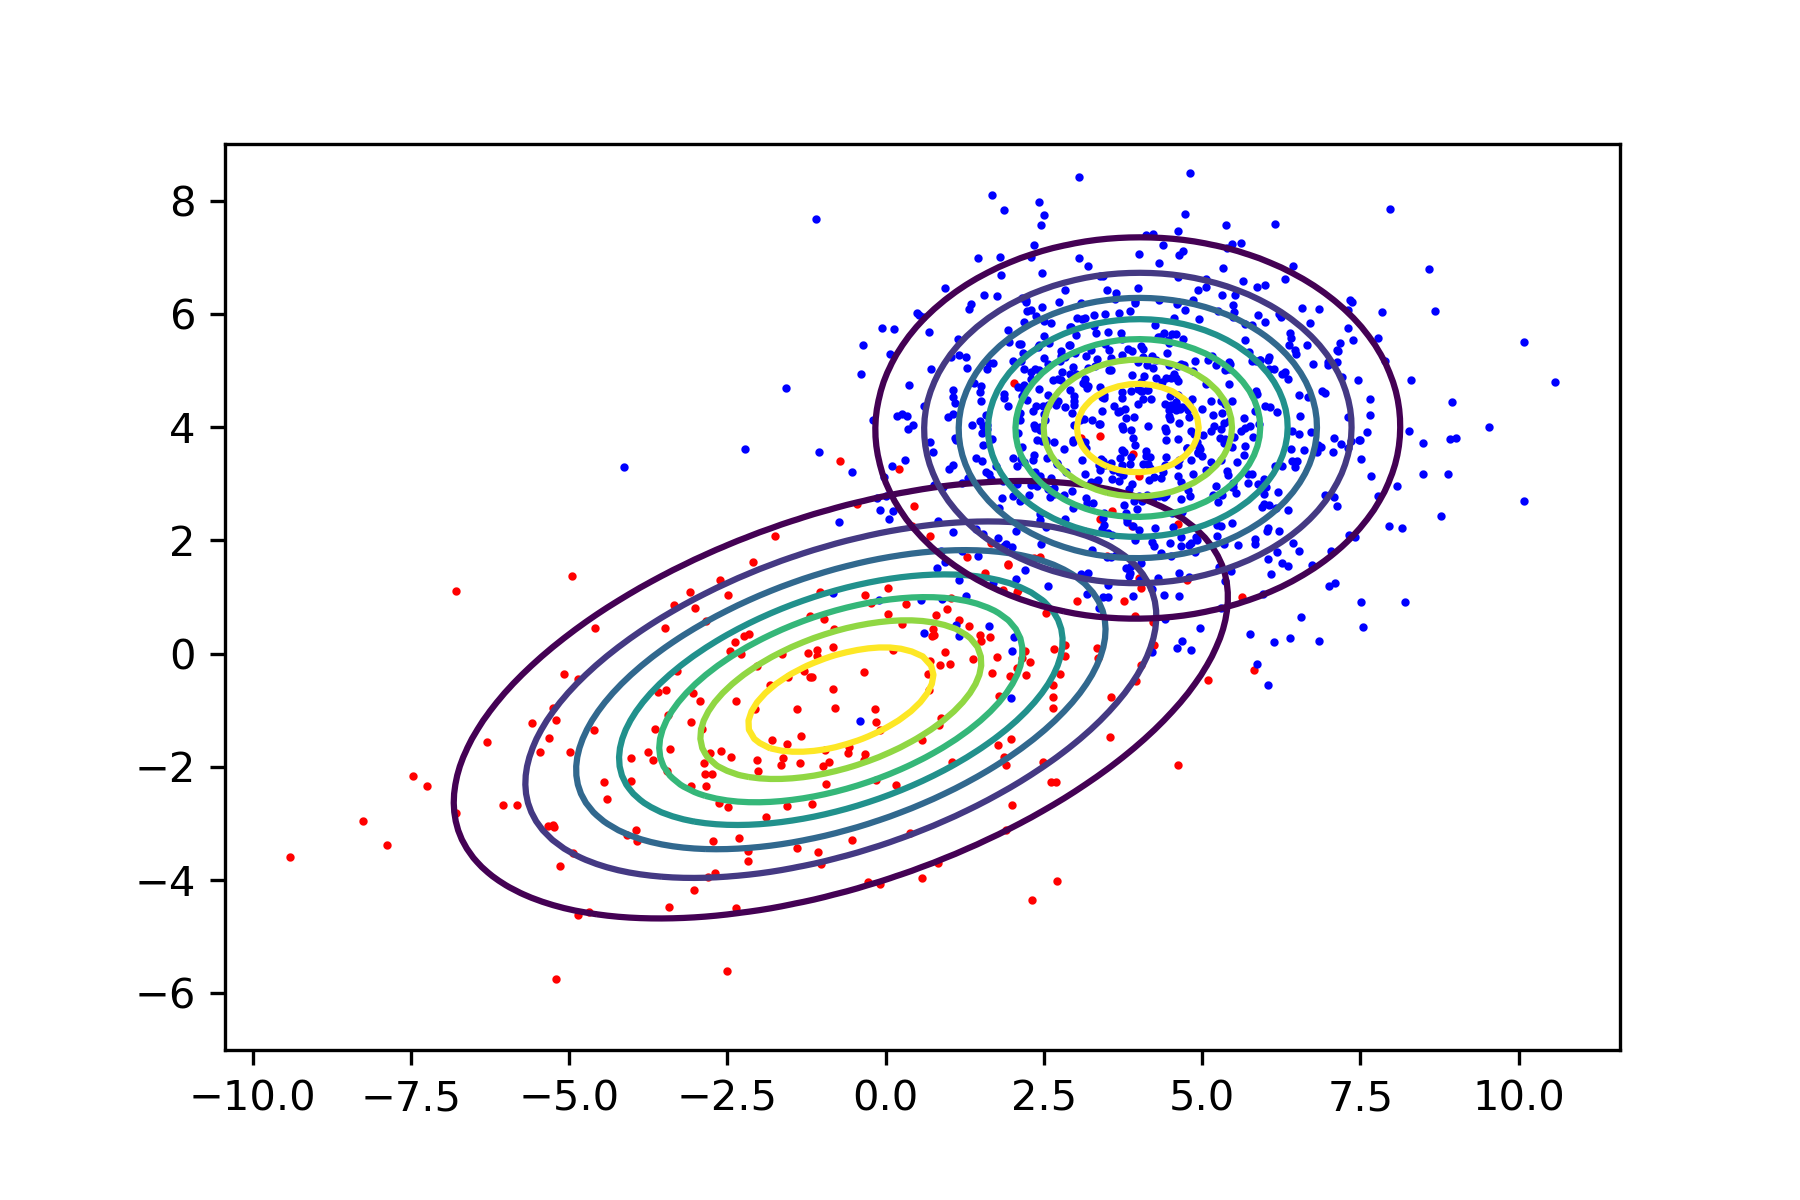
\includegraphics[width=0.8\linewidth]{pictures/plot_gaussians.png}
	\centering
	\caption{Plot of the class densities and data points.}
	\label{fig:densities}
\end{figure}
\begin{answer}
Using the unbiased estimates from before, we can plot the class densities and the data points. See Figure \ref{fig:densities} for the plot. According to the datasets, the red dots belong to class 1 and the blue dots belong to class 2.
\end{answer}

\end{question}

%----------------------------------------------

\begin{question}{Posterior}{8}
In a single graph, plot the posterior distribution of each class $p(C_i|x)$ and show the decision boundary. 
\begin{figure}[]
	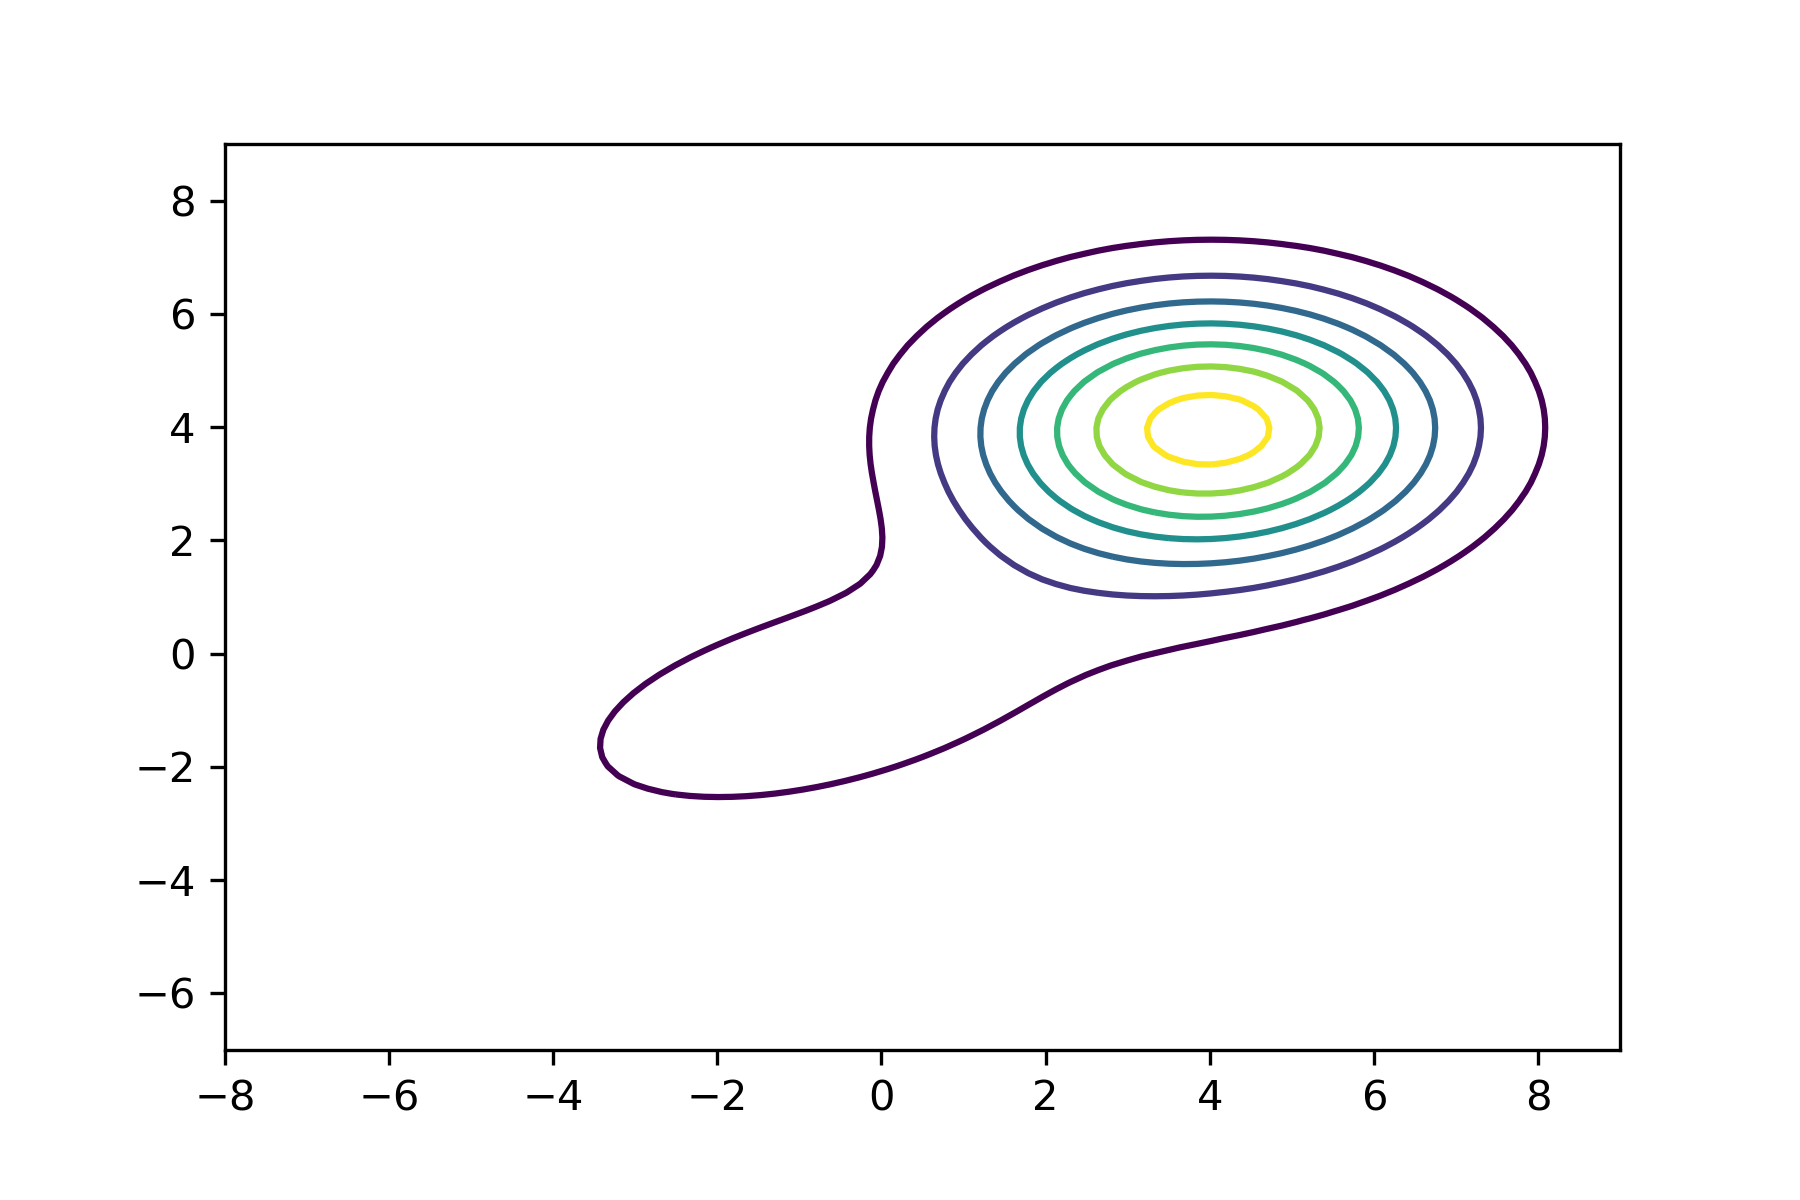
\includegraphics[width=0.8\linewidth]{pictures/posterior_contour.png}
	\centering
	\caption{Contour plot of the posterior distribution of each class in a single graph.}
	\label{fig:posterior_contour}
\end{figure}
\begin{figure}[]
	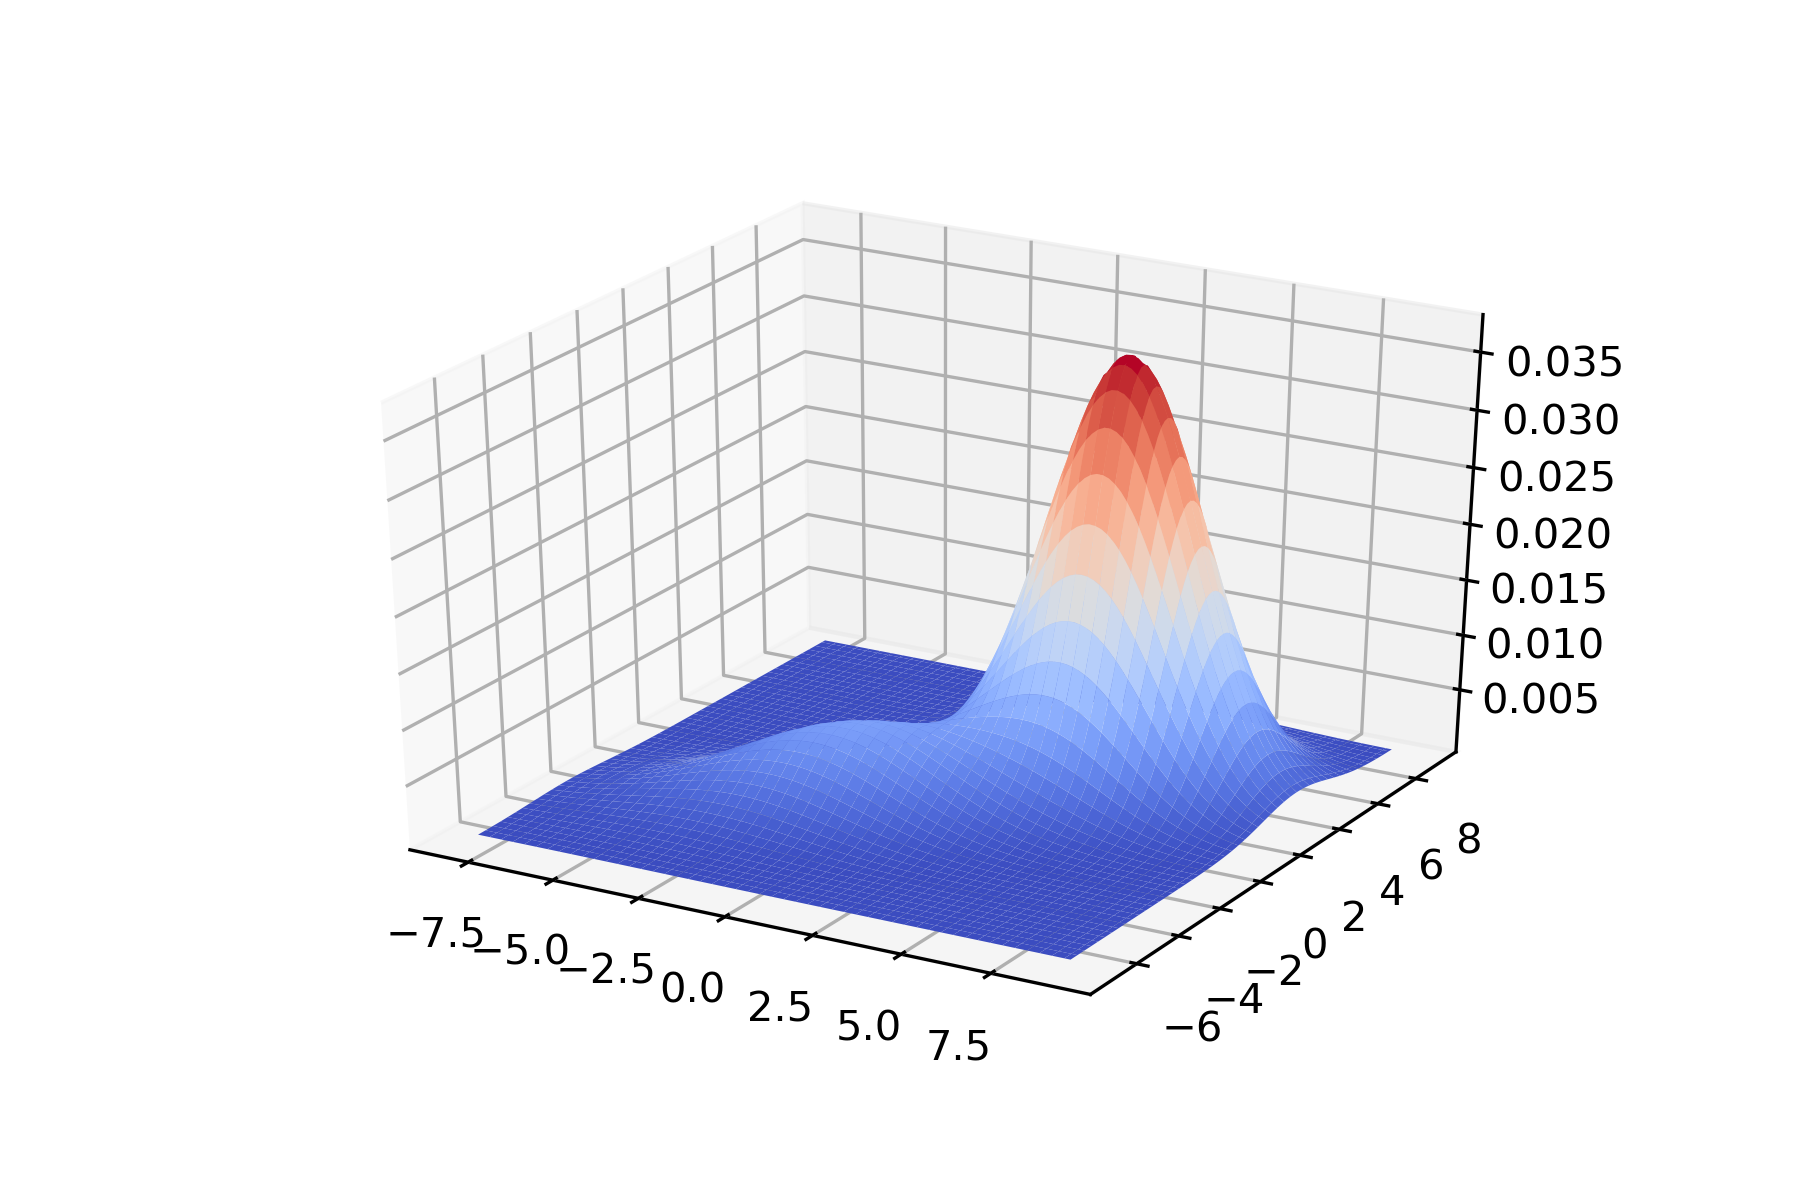
\includegraphics[width=0.8\linewidth]{pictures/posterior_3d.png}
	\centering
	\caption{3d plot of the posterior distribution of each class in a single graph.}
	\label{fig:posterior_3d}
\end{figure}
\begin{figure}[]
	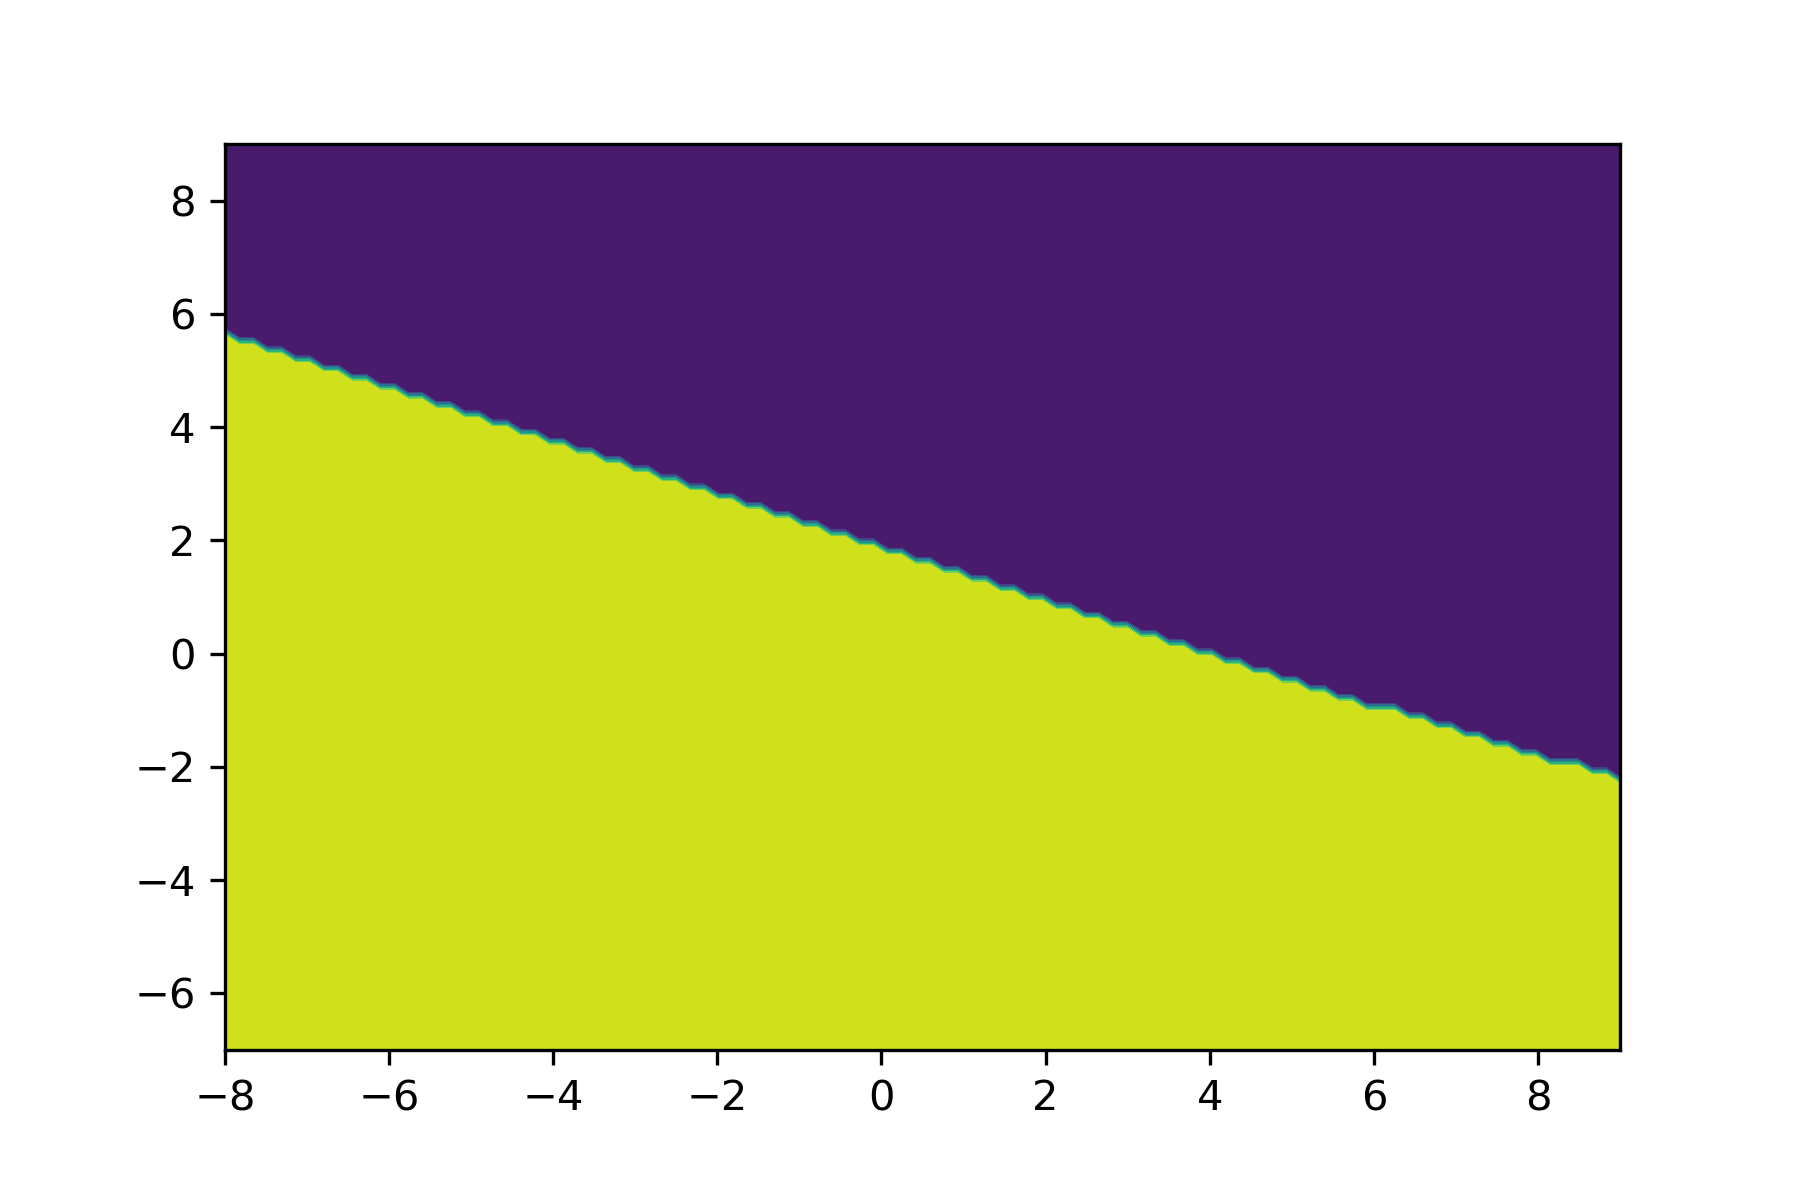
\includegraphics[width=0.8\linewidth]{pictures/decision_small.png}
	\centering
	\caption{Decision boundary with small scale of the x- and y-axes.}
	\label{fig:decision_small}
\end{figure}
\begin{figure}[]
	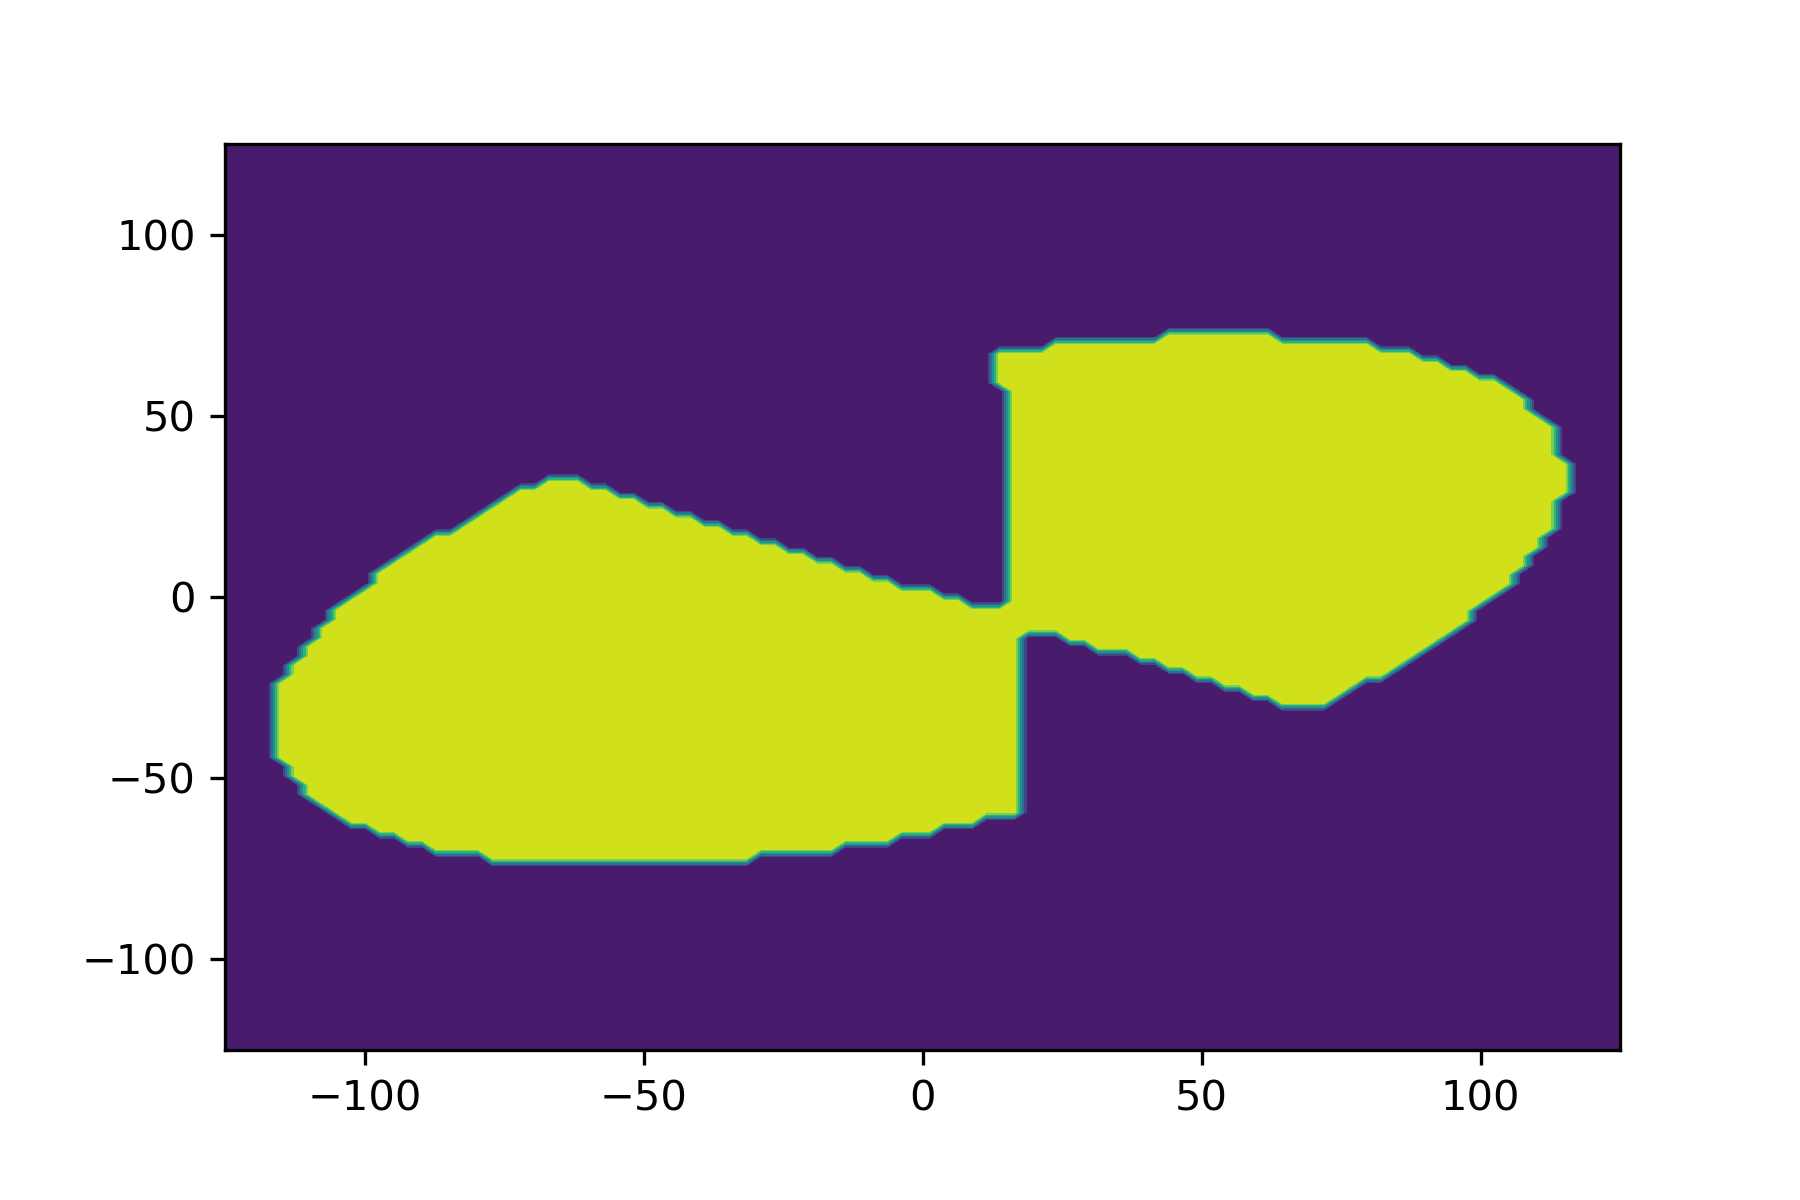
\includegraphics[width=0.8\linewidth]{pictures/decision_large.png}
	\centering
	\caption{Decision boundary with large scale of the x- and y-axes}
	\label{fig:decision_large}
\end{figure}
\begin{answer}
The figures \ref{fig:posterior_contour} and \ref{fig:posterior_3d} show the posterior distribution of both classes in a single plot. Figure \ref{fig:posterior_contour} shows a contour plot, whereas figure \ref{fig:posterior_3d} shows a 3d view.\\
The figures \ref{fig:decision_small} and \ref{fig:decision_large} display the decision boundary, with two different scales for the x- and y-axes. The colour yellow indicates a decision for class 1 and purple encodes a decision for class 2.
\end{answer}

\end{question}
\newpage
%----------------------------------------------

\begin{question}[bonus]{Bayesian Estimation}{15}
State the generic case of Bayesian linear regression with data $<\vec X, \vec Y>$ and parameters $\vec \theta$. What do we assume about the data, the model and the parameters?\\
Formulate the posterior distribution for your model parameters given the data, i.e., $p(\vec \theta | \vec X, \vec Y)$, and derive its mean and covariance, assuming that the model of the output variable is a Gaussian distribution with a fixed variance.\\
What do we do when we want to predict a new point?\\
Which are the advantages of being Bayesian? 

\begin{answer}
For this task we follow the these technical notes: Thomas P. Minka (2010) - Bayesian linear regression.\\
The data is is modeled in the following way: An input vector $\boldsymbol{x}$ of length $m$ multiplies a coefficient matrix $\boldsymbol{\theta}$ in order to produce and output vector $\boldsymbol{y}$ of length $d$, with Gaussian noise $\boldsymbol{e}$ added. The noise $\boldsymbol{e}$ has zero mean and a variance $\mathbf{V}$.\\
\begin{equation*}
\begin{aligned} \mathbf{y} &=\mathbf{\boldsymbol{\theta} x}+\mathbf{e} \\ \mathbf{e} & \sim \mathcal{N}(0, \mathbf{V})  \end{aligned}
\end{equation*}
This is equivalent to the following conditional distribution for $\mathbf{y}$:
\begin{equation*}
p(\mathbf{y} | \mathbf{x}, \boldsymbol{\theta}, \mathbf{V})  \sim \mathcal{N}(\boldsymbol{\theta} \mathbf{x}, \mathbf{V})
\end{equation*}
The set of pairs $D=\{(\mathbf{y}_{1}, \mathbf{x}_{1}), \ldots,(\mathbf{y}_{N}, \mathbf{x}_{N})\}$ are independent and identically distributed, which leads to:
\begin{equation}
\begin{aligned} 
p(\mathbf{Y} | \mathbf{X}, \boldsymbol{\theta}, \mathbf{V})&=\prod_{i} p(\mathbf{y}_{i} | \mathbf{x}_{i}, \boldsymbol{\theta}, \mathbf{V})
\\ &=\frac{1}{|2 \pi \mathbf{V}|^{N / 2}} \exp (-\frac{1}{2} \operatorname{tr}(\mathbf{V}^{-1}[\boldsymbol{\theta} \mathbf{X} \mathbf{X}^{\mathrm{T}} \boldsymbol{\theta}^{\mathrm{T}}-2 \mathbf{Y} \mathbf{X}^{\mathrm{T}} \boldsymbol{\theta}^{\mathrm{T}}+\mathbf{Y} \mathbf{Y}^{\mathrm{T}}]))
\end{aligned} 
\label{eq:likelihood}
\end{equation}
A conjugate prior for the coeffiecients $\boldsymbol{\theta}$ is the matrix-normal density with parameters $\mathbf{M}$($dxm$), $\mathbf{V}$($dxd$) and $\mathbf{K}$($mxm$):
\begin{equation}
\begin{aligned} p(\boldsymbol{\theta}) & \sim \mathcal{N}(\mathbf{M}, \mathbf{V}, \mathbf{K}) \\ &=\frac{|\mathbf{K}|^{d / 2}}{|2 \pi \mathbf{V}|^{m / 2}} \exp (-\frac{1}{2} \operatorname{tr}((\boldsymbol{\theta}-\mathbf{M})^{\mathrm{T}} \mathbf{V}^{-1}(\boldsymbol{\theta}-\mathbf{M}) \mathbf{K})) \end{aligned}
\label{eq:prior}
\end{equation}
If we use the following abbreviations:
\begin{equation*}
\mathbf{S}_{x x}=\mathbf{X} \mathbf{X}^{\mathrm{T}}+\mathbf{K}
\end{equation*}
\begin{equation*}
\mathbf{S}_{y x}=\mathbf{Y} \mathbf{X}^{\mathrm{T}}+\mathbf{M K}
\end{equation*}
\begin{equation*}
\mathbf{S}_{y y}=\mathbf{Y} \mathbf{Y}^{\mathrm{T}}+\mathbf{M K M}^{\mathrm{T}}
\end{equation*}
\begin{equation*}
\mathbf{S}_{y | x}=\mathbf{S}_{y y}-\mathbf{S}_{y x} \mathbf{S}_{x x}^{-1} \mathbf{S}_{y x}^{\mathrm{T}}
\end{equation*}
Under the assumption that the output is gaussian with fixed variance, he posterior for $\boldsymbol{\theta}$ then is matrix normal:
\begin{equation*}
p(\boldsymbol{\theta}| D, \mathbf{V}) \sim \mathcal{N}(\mathbf{S}_{y x} \mathbf{S}_{x x}^{-1}, \mathbf{V}, \mathbf{S}_{x x})
\end{equation*}
This can be derived by taking the likelihood (\ref{eq:likelihood}) times the conjugate prior (\ref{eq:prior}):
\begin{equation*}
\begin{aligned} p(\mathbf{Y}, \boldsymbol{\theta} | \mathbf{X}, \mathbf{V}) & \propto \exp (-\frac{1}{2} \operatorname{tr}(\mathbf{V}^{-1}(\boldsymbol{\theta} \mathbf{S}_{x x} \boldsymbol{\theta}^{\mathrm{T}}-2 \mathbf{S}_{y x} \boldsymbol{\theta}^{\mathrm{T}}+\mathbf{S}_{y y}))) \\ & \propto \exp (-\frac{1}{2} \operatorname{tr}(\mathbf{V}^{-1}((\boldsymbol{\theta}-\mathbf{S}_{y x} \mathbf{S}_{x x}^{-1}) \mathbf{S}_{x x}(\boldsymbol{\theta}-\mathbf{S}_{y x} \mathbf{S}_{x x}^{-1})^{\mathrm{T}}+\mathbf{S}_{y | x}))) \end{aligned}
\end{equation*}

The advantages of being Bayesian are, that the pararameters are regarded as random variables and a prior is put on these. As a consequence the uncertainty of parameter values is incorporated in the model. This leads to automatic regularization and model selection according to the data and avoids over-/ or underfitting. There is no need for separate model selection criteria as BIC and AIC. Furthermore bayesian estimation provides a natural way of  including prior knowledge with incoming data, in order to obtain a posterior. This posterior can be used as prior for new decisions.
\end{answer}

\end{question}

\end{questions}

	
	\newif\ifvimbug
\vimbugfalse

\ifvimbug
\begin{document}
\fi

\exercise{Non-parametric Density Estimation}
 
In this exercise, you will use the datasets \texttt{nonParamTrain.txt} for training and \texttt{nonParamTest.txt} for evaluating the performance of your model.

\begin{questions}

%----------------------------------------------

\begin{question}{Histogram}{4}
Compute and plot the histograms using $0.02$, $0.5$, $2.0$ size bins of the training data.  
Intuitively, indicate which bin size performs the best and explain why. Knowing only these three trials, would you be sure that the one you picked is truly the best one? Attach the plot of the histograms and a snippet of your code.

\begin{answer}
The first figure \ref{fig:histogram1} shows a Histogram of the data with bin size 0.02. The "spicky" behavior and empty bins which are conssistend throughout the Histogram, indicate that the bin size has been chosen to to small (to much Variance).	

In the next Figure \ref{fig:histogram2} you can imagine a trend for the underlying distribution. This indicates a good bin size.


The third histogram \ref{fig:histogram3} also schows a trend of the underlying function, but compared to figure \ref{fig:histogram2} some of details get lost in the representation. Meaning that the bin size has been choosen to big (to much Bias).

Bonus: This last histogram \ref{fig:histogram4} is an histogram with the number of bins determined by Sturges Rule. It's shape is similiar to figure (2), only beeing a bit more smooth. However Sturges rule is critized to smooth the Histogram to much (Hyndman, 1995) and should be only used as a rule of thumb. In this case it adds futher believe into a bin size of about 0.5

However in the end for these four bin sizes, we cant be completly sure that the one choose is the best, but we have atleast good evidence for it.
	
\end{answer}
\end{question}


\begin{figure}[H]
	\centering
	\begin{subfigure}[b]{0.4\linewidth}
		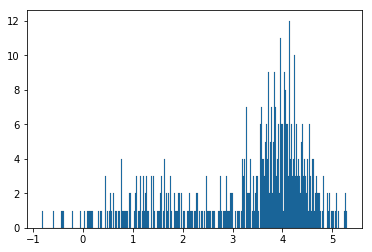
\includegraphics[width=\linewidth]{pictures/histogram002.png}
		\caption{Bin Size 0.02.}
		\label{fig:histogram1}
	\end{subfigure}
	\begin{subfigure}[b]{0.4\linewidth}
		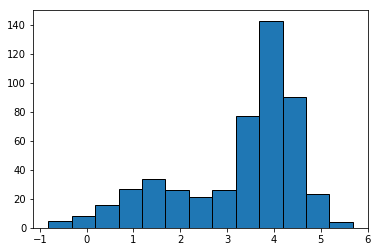
\includegraphics[width=\linewidth]{pictures/histogram05.png}
		\caption{Bin Size 0.5.}
		\label{fig:histogram2}
	\end{subfigure}
	\caption{First two Histograms}
\end{figure}

\begin{figure}[H]
	\centering
	\begin{subfigure}[b]{0.4\linewidth}
		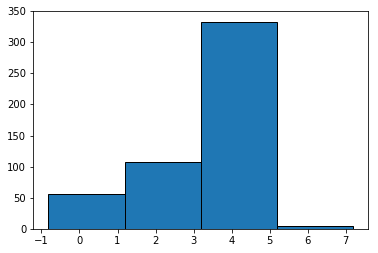
\includegraphics[width=\linewidth]{pictures/histogram2.png}
		\caption{Bin Size 2}
		\label{fig:histogram3}
	\end{subfigure}
	\begin{subfigure}[b]{0.4\linewidth}
		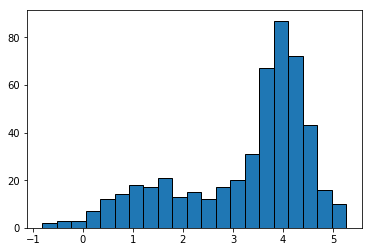
\includegraphics[width=\linewidth]{pictures/histogramSturge.png}
		\caption{Bin size calculated with Sturges Rule.}
		\label{fig:histogram4}
	\end{subfigure}
	\caption{Last two Histograms}
	
\end{figure}

	
Snippet of the code used: 
\begin{lstlisting}{}
import numpy as np
train = np.loadtxt("nonParamTrain.txt");

import matplotlib.pyplot as plt
binwidth = 0.02
bin_sequence = np.arange(min(train), max(train) + binwidth, binwidth)  
plt.hist(train, bins=bin_sequence, edgecolor="black" ,linewidth=0.1);
\end{lstlisting}

%----------------------------------------------

\begin{question}{Kernel Density Estimate}{6}
Compute the probability density estimate using a Gaussian kernel with $\sigma=0.03$, $\sigma=0.2$ and $\sigma=0.8$ of the training data. Compute the log-likelihood of the data for each case, compare them and show which parameter performs the best.
Generate a single plot with the different density estimates and attach it to your solutions. Plot the densities in the interval $x \in [-4,8]$, attach a snippet of your code and comment the results.

\begin{answer}\end{answer}

\end{question}

%----------------------------------------------

\begin{question}{K-Nearest Neighbors}{6}
Estimate the probability density with the K-nearest neighbors method with $K=2, K=8, K=35$.
Generate a single plot with the different density estimates and attach it to your solutions. Plot the densities in the interval $x \in [-4,8]$, attach a snippet of your code and comment the results.

\begin{answer}\end{answer}

\end{question}

%----------------------------------------------

\begin{question}{Comparison of the Non-Parametric Methods}{4}
Estimate the log-likelihood of the testing data using the KDE estimators and the K-NN estimators.
Why do we need to test them on a different data set? Compare the log-likelihoods of the estimators w.r.t. both the training and testing sets in a table. Which estimator would you choose?

\begin{answer}\end{answer}

\end{question}

\end{questions}

	
	\newif\ifvimbug
\vimbugfalse

\ifvimbug
\begin{document}
\fi

\exercise{Expectation Maximization}
 
In this exercise, you will use the datasets \texttt{gmm.txt}. It contains data from a Gaussian Mixture Model with four 2-dimensional Gaussian distributions.

\begin{questions}

%----------------------------------------------

\begin{question}{Gaussian Mixture Update Rules}{2}
Define the model parameters and the update rules for your model. 
Specify the E- and M-steps of the algorithm.

\begin{answer}\end{answer}

\end{question}

%----------------------------------------------

\begin{question}{EM}{18}
Implement the Expectation Maximization algorithm for Gaussian Mixture Models. Initialize your model uniformly. Generate plots at different iterations $t_i \in [1,3,5,10,30]$, showing the data and the mixture components, and plot the log-likelihood for every iteration $t_i=1:30$. Attach a snippet of your code.

\begin{answer}\end{answer}

\end{question}

\end{questions}


\end{document}
